\documentclass[12pt]{article}
\usepackage[utf8]{inputenc}
\usepackage[a4paper,margin=0.4in]{geometry}
\usepackage{amsmath} 
\usepackage{graphicx}
\usepackage{float}
\usepackage{multirow}
\usepackage{tabularx} 
\usepackage{caption}
\usepackage{enumitem}
\usepackage{subcaption}
\usepackage{array}
\usepackage[numbered]{matlab-prettifier}
\usepackage{pgf}
\usepackage{pgfpages}
\usepackage[table,xcdraw]{xcolor}

\pgfpagesdeclarelayout{boxed}
{
  \edef\pgfpageoptionborder{0pt}
}
{
  \pgfpagesphysicalpageoptions
  {%
    logical pages=1,%
  }
  \pgfpageslogicalpageoptions{1}
  {
    border code=\pgfsetlinewidth{2pt}\pgfstroke,%
    border shrink=\pgfpageoptionborder,%
    resized width=.95\pgfphysicalwidth,%
    resized height=.95\pgfphysicalheight,%
    center=\pgfpoint{.5\pgfphysicalwidth}{.5\pgfphysicalheight}%
  }%
}
\pgfpagesuselayout{boxed}

\title{

    Indian Institute Of Technology Madras
    \begin{figure}[htp]
        \centering
        \includegraphics[width=6cm]{Pics/IITM logo.png}
    \end{figure}
    \begin{center}
        \textbf{\\ID5130 Parallel Scientific Computing\\}
        
       Assignment 1
    \end{center}
}
\author{
    AE20B027 Hareesh P Nair\\ 
}
\date{}

\begin{document}
\pagenumbering{gobble}
\maketitle
\newpage
\pagenumbering{arabic}


%\listoffigures
\newpage

\section*{Question 1}
Solve the following system of linear equations using recursive-doubling algorithm by clearly showing all the required steps. You may use the recursive expressions that we have developed or solve it directly using the philosophy of the method

$$3x_1 - x_2 = 2$$
$$-x_1+3x_2-x_3=1$$
$$-x_2+3x_3-x_4=1$$
$$-x_3+3x_4=2$$

\subsection*{Solution}

Consider the given equations be labelled as:
\begin{equation}
    3x_1 - x_2 = 2
    \label{eq1}
\end{equation}

\begin{equation}
    -x_1+3x_2-x_3=1
    \label{eq2}
\end{equation}

\begin{equation}
    -x_2+3x_3-x_4=1
    \label{eq3}
\end{equation}

\begin{equation}
    -x_3+3x_4=2
    \label{eq4}
\end{equation}

\noindent Consider equation \eqref{eq1} and \eqref{eq2}, from equation \eqref{eq2}, we get
$$x_2 = \frac{1+x_1+x_3}{3}$$
\noindent Substituting value of $x_2$ in equation \eqref{eq1}, we get
$$3x_1 - \left( \frac{1+x_1+x_3}{3}\right) = 2$$
\noindent Multiplying the above equation by $3$, we get
\begin{equation}
    8x_1-x_3 = 7
    \label{eq5}
\end{equation}

\noindent Now consider equation \eqref{eq1}, \eqref{eq2} and \eqref{eq3},

$$x_1 = \frac{2+x_2}{3} \text{\ \ from equation \eqref{eq1}}$$

$$x_3 = \frac{1+x_2+x_4}{3} \text{\ \ from equation \eqref{eq3}}$$

\noindent Substituting them in equation \eqref{eq2} and multiplying by 3, we get
\begin{equation}
    7x_2 - x_4 = 6
    \label{eq6}
\end{equation}

\noindent Now consider equation \eqref{eq2}, \eqref{eq3} and \eqref{eq4},

$$x_2 = \frac{1+x_3+x_4}{3} \text{\ \ from equation \eqref{eq2}}$$

$$x_4 = \frac{2+x_3}{3} \text{\ \ from equation \eqref{eq4}}$$

\noindent Substituting them in equation \eqref{eq2} and multiplying by 3, we get
\begin{equation}
    7x_3 - x_1 = 6
    \label{eq7}
\end{equation}

\noindent Consider equation \eqref{eq3} and \eqref{eq4}
$$x_3 = \frac{1+x_2+x_4}{3} \text{\ \ from equation \eqref{eq3} }$$

substituting in equation \eqref{eq4} and multiplying by 3, we get 
\begin{equation}
    8x_4-x_2 = 7
    \label{eq8}
\end{equation}

\noindent Now consider equation \eqref{eq5} and \eqref{eq7},
$$x_3 = 8x_1 - 7$$
\noindent Substituting in equation \eqref{eq7}, we get $x_1 = 1$

\noindent Similarly considering equation \eqref{eq6} and \eqref{eq8}, we get $x_2 = 1$

\noindent Similarly considering equation \eqref{eq5} and \eqref{eq7} again, we get $x_3 = 1$

\noindent Lastly, considering equation \eqref{eq6} and \eqref{eq8} again, we get $x_4 = 1$

\noindent Hence, 
$$
\boxed{x_1 =1} \quad \boxed{x_2 = 1} \quad \boxed{x_3 = 1} \quad \boxed{x_4 = 1}
$$

\section*{Question 2}

Consider the calculation of the derivative of the following function,
$$
f(x) = \sin(5x) \quad 0\leq x \leq 3
$$
using four-order accurate Padé scheme for the interior and third-order accurate one-sided Padé scheme near the boundaries, given as follows,

$$
f_{j+1}'+4f_{j}'+f_{j-1}' = \frac{3}{h}\left(f_{j+1} - f_{j-1}\right)
$$

where $j$ is any interior point $( j = 1, 2, . . . , n - 1)$ and
$$
f_0'+2f_1' = \frac{1}{h}\left( -\frac{5}{2}f_0 + 2f_1 + \frac{1}{2}f_2\right)
$$

$$
f_n'+2f_{n-1}' = \frac{1}{h}\left( -\frac{5}{2}f_n - 2f_{n-1} + \frac{1}{2}f_{n-2}\right)
$$
where $h$ is the grid spacing and $n$ is the number of grid points in the $x$ direction.
\begin{enumerate}[label=\alph*]
    \item Develop a serial program to compute the derivative using the tridiagonal LU decomposition. Plot the analytical solution and the numerical solution obtained for $n$ = 25.
    \item Develop an OpenMP program to compute the derivative using the recursive-doubling algorithm. Plot the analytical solution and the numerical solution for $n = 100$ and number of threads $p = 2$. Plot the time-taken by the solver for $n = 1000$ for number of threads $p = 2, 4 \text{\ and\ } 8$.
\end{enumerate}

\newpage
\subsection*{Solution - a}

The serial code has been developed in C++ and uploaded to the relevant submission link. The plot for the four-order Padé scheme is obtained from the code is given below

\begin{figure}[!ht]
    \centering
    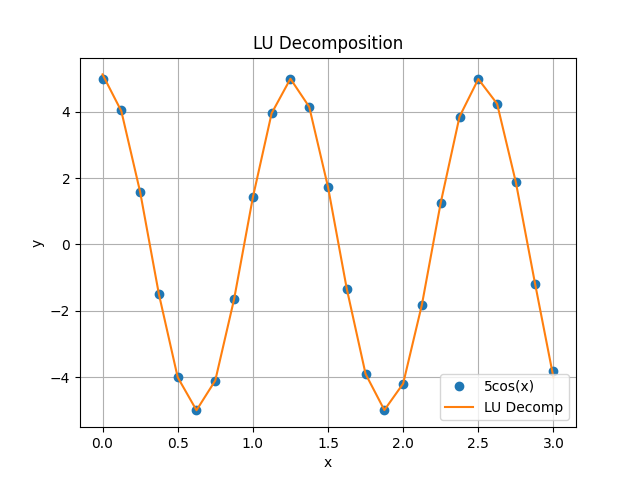
\includegraphics[width = 0.55\linewidth]{Pics/Pade_LU_Decomp.png}
    \caption{Plot of four-order Padé scheme solution using LU Decomposition}
    \label{fig:LUD}
\end{figure}

\subsection*{Solution - b}

\noindent The code for the Recursive Doubling method for solving the Padé scheme has been developed and uploaded. The plot for the Recursive Doubling solution for $n=100$ is given below:

\begin{figure}[!ht]
    \centering
    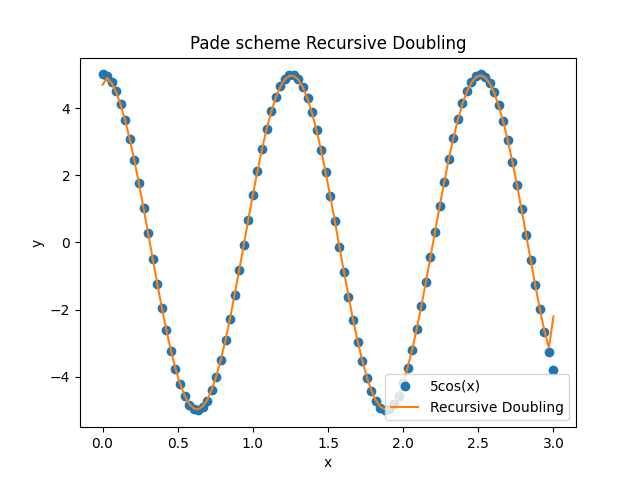
\includegraphics[width = 0.55\linewidth]{Pics/Pade_scheme_RecursiveDoubling.png}
    \caption{Plot of four-order Padé scheme solution using Recursive Doubling}
    \label{fig:RD}
\end{figure}

\noindent The plot of time taken for different number of threads $p=2,4 \text{\ and \ } 8$ for solving the Recursive Doubling algorithm is given below:

\begin{figure}[!ht]
    \centering
    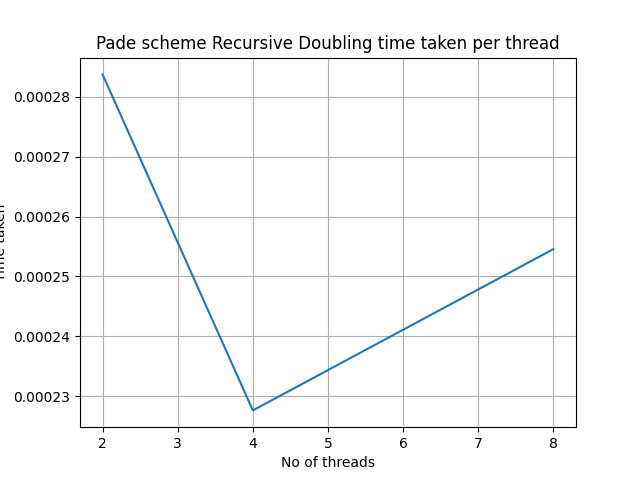
\includegraphics[width = 0.55\linewidth]{Pics/Pade_scheme_RecursiveDoubling_time_taken.png}
    \caption{Time taken for different number of threads to solve Recursive Doubling algorithm}
    \label{fig:RD_time}
\end{figure}
\newpage
\noindent In the above plot, we can see that for $p=8$, the time taken is more than for $p=4$. This can be explained by the overhead time taken by 8 threads to be initialized is itself more than the calculation of the algorithm by 8 threads. Hence, we get this trend. In cases where the number of points used of discretization, $n$, is much higher, we can avoid such scenarios.

\section*{Question 3}

Consider the solution of the following Poisson equation,
$$
\nabla^2 \phi = -q; \quad q = 2(2-x^2-y^2); \quad \phi(\pm 1, y) = 0; \quad \phi(x, \pm 1) = 0 
$$
using Gauss-Seidel method. The discretized equation using this method can be written as follows,
$$
\phi_{i,j}^{(k+1)} = \frac{1}{4}\left[\phi_{i+1,j}^{(k)} + \phi_{i-1,j}^{(k+1)} + \phi_{i,j+1}^{(k)} + \phi_{i,j-1}^{(k+1)} \right] + \frac{\Delta^2}{4}q_{i,j}
$$
where $\Delta = \Delta x = \Delta y$. Consider an initial guess of $\phi(x,y)= 0$  everywhere. The exact solution to this problem is given by $\phi = (x^2 - 1) (y^2 - 1)$. Use double precision arithmetic.

\begin{enumerate}[label=\alph*]
    \item Develop a serial Gauss-Seidel program to solve the discretized equations and solve the system using $\Delta = \Delta x = \Delta y = 0.1$ (that is 21 points along each of the directions). Report the number of iterations required to bring the numerical solution to within 1$\%$ of the exact solution. Plot the numerical and the analytical solutions of $\phi$ vs $x$ for $y = 0.5$.
    \item Develop an OpenMP program for Gauss-Seidel method using the (i) diagonal approach (ii) red-black coloring approach.
    \item For each of the parallel programs developed above, verify that your parallel program is giving the same result as that of the serial program that you developed above for a grid of $\Delta = 0.1$ by plotting the two results on the same graph. Upon successful verification, run this program for $\Delta = 0.1, \ 0.01, \text{and \ } 0.005$ using 8 threads.  Plot the time-taken by the parallel solvers and the serial solver as a function of the grid size ($\Delta$). Do you see any improvement in performance? Which parallel method is better ?
    \item For a grid size of $\Delta = 0.005$, plot the time-taken by each of the parallel solvers as a function of the number of threads. Consider the number of threads to be $p = 2, 4, 8\ \text{and \ } 16$. Which parallel method is better?
\end{enumerate}

\subsection*{Solution - a}

\noindent The serial code for Gauss Seidel has been developed in C++ and the following plot was obtained for the Gauss Seidel serial scheme for $\Delta = 0.1$ 
\begin{figure}[!ht]
    \centering
    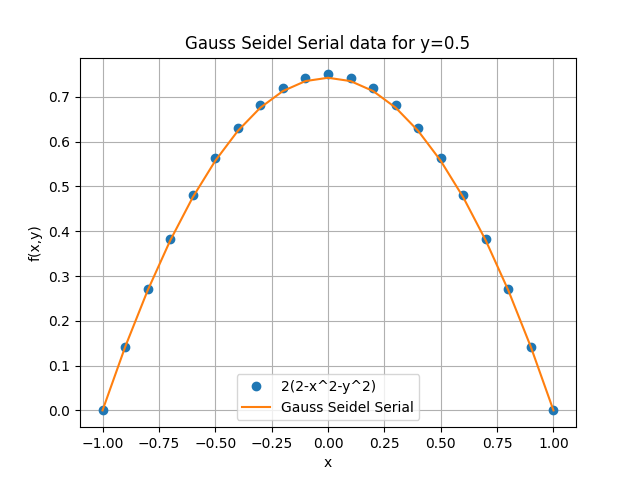
\includegraphics[width = 0.55\linewidth]{Pics/Gauss_Seidel_Serial.png}
    \caption{Plot of $\phi(x,y=0.5)$ for Gauss Seidal scheme solution}
    \label{fig:GS}
\end{figure}
\vspace{-2mm}
\subsection*{Solution - b}
\noindent The code for the Diagonal Wave method and Red Black coloring for solving the Gauss Seidel scheme has been developed using C++ and uploaded to the relevant submission link. The following set of answers will dive into more detail about them

\subsection*{Solution - c}

\noindent The values of the Diagonal Wave method and Red-Black coloring method is closely matching with the serial solution for $\phi(x,y=0.5)$. This can be visulaized in the below plot
\begin{figure}[!ht]
\vspace{-5mm}

    \centering
    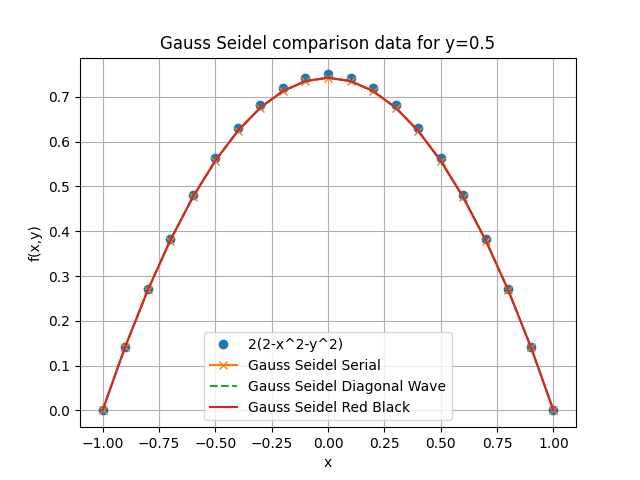
\includegraphics[width = 0.55\linewidth]{Pics/Gauss_Seidel_comparison.png}
    \caption{Plot of $\phi(x,y=0.5)$ using different algorithm for Gauss Seidel scheme}
    \label{fig:GS_compare}
\end{figure}


\noindent Now that the result of the parallel programs has been verified, the time taken by each parallel program for solving the Poisson equation by following different algorithm on Gauss Seidel method for different grid sizes $\Delta = 0.1, \ 0.01, \  \text{and} \ 0.005 $ for $p = 8$ is recorded. The following plot can provide a visualisation on the time taken
\begin{figure}[!ht]
    \centering
    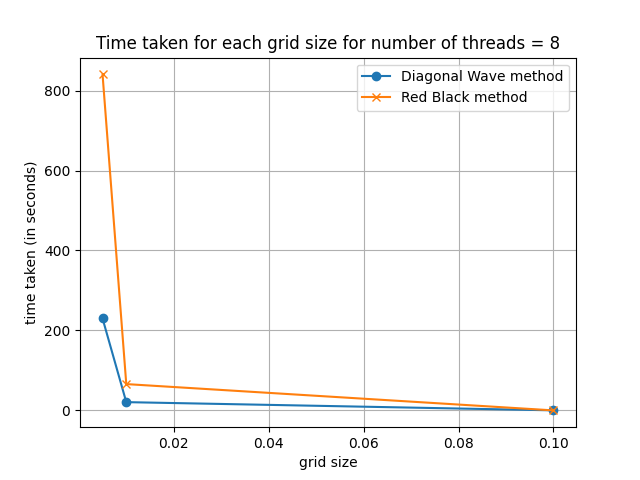
\includegraphics[width = 0.55\linewidth]{Pics/TimeVsGridSize_comparison.png}
    \caption{Time taken for 8 threads to perform Gauss Seidel on different grid sizes}
    \label{fig:GS_grid_time}
\end{figure}

\vspace{-5mm}
\noindent As we can see from the above plot, the time taken by each algorithm is different for each grid sizes. From observation we can say \textbf{Diagonal Wave method performs much faster than Red Black coloring method} for $p =8$ number of threads. Also the time taken for smaller grid size is much higher than the time taken for a larger grid size.

\subsection*{Solution - d}
The following plot was obtained for the time taken for solving the Poisson equation by the Gauss Seidel iteration method using different algorithms for $\Delta = 0.005$ and $p=2,4, \text{and}, 8$. (Note: \textbf{I cannot use 16 threads as my laptop is hexacore}).

\begin{figure}[!ht]
    \centering
    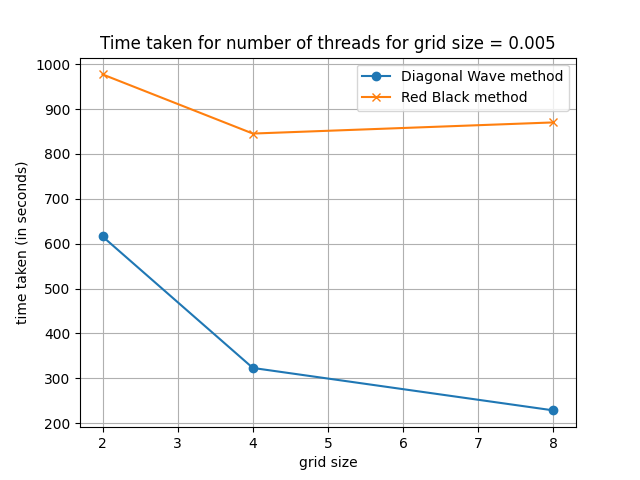
\includegraphics[width = 0.55\linewidth]{Pics/TimeVsNoOfThreads_comparison.png}
    \caption{Time taken for different number of  threads to perform Gauss Seidel with grid size = 0.005}
    \label{fig:GS_thread_time}
\end{figure}

\noindent From the plot, its obvious that \textbf{Diagonal Wave Method} is performing much faster compared to Red-Black-coloring scheme

\end{document}